%是否有ppt笔?
%一般时间多久

%ctrl+L  幻灯片播放

%LaTeX手动安装宏包(package)以及生成帮助文档的整套流程
%https://www.cnblogs.com/csucat/p/5142459.html
%https://www.ctan.org/pkg/

%一、要对论文的内容进行概括性的整合,将论文分为引言和试验设计的目的意义、材料和方法、结果、讨论、结论、致谢几部分。
%
%二、在每部分内容的presentation中,原则是:图的效果好于表的效果,表的效果好于文字叙述的效果。最忌满屏幕都是长篇大论,让评委心烦。能引用图表的地方尽量引用图表,的确需要文字的地方,要将文字内容高度概括,简洁明了化,用编号标明。
%三、
%1 文字版面的基本要求
%幻灯片的数目:硕士答辩20min 20~35张
%硕士答辩10min 10~20张
%博士答辩30min 30~50张
%字号字数行数:标题44号(40)
%正文32号(不小于24号字)
%每行字数在20~25个
%每张PPT 6~7行 (忌满字)
%中文用宋体(可以加粗),英文用 Time New Romans
%对于PPT中的副标题要加粗
%PPT中的字体颜色不要超过3种(字体颜色要与背景颜色反差大)
%建议新手配色:(1)白底,黑、红、篮字
%(2)蓝底,白、黄字(浅黄或橘黄也可)
%添加图片格式:好的质量图片TIF格式,GIF图片格式最小
%图片外周加阴影或外框效果比较好
%PPT总体效果:图片比表格好,表格比文字好;动的比静 的好,无声比有声好。
%
%四、(注意)
%幻灯片的内容和基调。背景适合用深色调的,例如深蓝色,字体用白色或黄色的黑体字,显得很庄重。值得强调的是,无论用哪种颜色,一定要使字体和背景显成 明显反差。 注意:要点!用一个流畅的逻辑打动评委。字要大:在昏暗房间里小字会看不清,最终结果是没人听你的介绍。不要用PPT自带模板:自带模板那些评委们都见 过,且与论文内容无关,要自己做,简单没关系,纯色没关系,但是要自己做! 时间不要太长:20分钟的汇报,30页内容足够,主要是你讲,PPT 是辅助性的。 记得最后感谢母校,系和老师,弄得煽情点 ^_^ 。

\documentclass{beamer}
\usepackage[UTF8]{ctex}

%metropolis Boadilla Madrid CambridgeUS JuanLesPins
\usetheme{Madrid}
% 这里还可以选择别的主题Bergen,Boadilla,Madrid,AnnArbor, CambridgeUS,Pittsburgh
% Rochester. 有导航栏的Antibes,JuanLesPins,Montpellier,有内容的Berkeley,PaloAlto,
% Goettingen,Marburg,Hannover,有最小导航栏的Berlin,Ilmenau,Dresden,Darmstadt,
% Frankfurt,Singapore,Szeged,有章和节表单的Copenhagen,Luebeck,Malmoe,Warsaw


%\usecolortheme{default}
% 这个主题一般选择动物来命名
% 这里还可以选择别的颜色主题,如默认的和有特别目的的颜色主题default,structure,sidebartab,全颜色主题albatross,
% beetle,crane,dove,fly,seagull,wolverine,beaver
%%%%%%%%%%%%%%%%%%%%%%%%%%%%%%%%%%%%%%%%%%%%%%%%%%%%%%%%%%%%%%%%%%%%%%%%%%%%%%%%%%%%%%%%%%%%%%%%%%%%%%%%

%%%%%%%%%%%%%%%%%%%%%%%设置内部颜色主题(这些主题一般改变block 里的颜色)%%%%%%%%%%%%%%%%%%%%%%%%%%%%%%%%%%

%\usecolortheme{orchid}
% 这个主题一般选择植物来命名
% 这里还可以选择别的颜色主题,如默认的和有特别目的的颜色主题lily,orchid,rose
%%%%%%%%%%%%%%%%%%%%%%%%%%%%%%%%%%%%%%%%%%%%%%%%%%%%%%%%%%%%%%%%%%%%%%%%%%%%%%%%%%%%%%%%%%%%%%%%%%%%%%%%

%%%%%%%%%%%%%%%%%%%%%%%设置外部颜色主题(这些主题一般改变title 里的颜色)%%%%%%%%%%%%%%%%%%%%%%%%%%%%%%%%%%
%\usecolortheme{whale}
% 这个主题一般选择海洋动物来命名
% 这里还可以选择别的颜色主题,如默认的和有特别目的的颜色主题whale,seahorse,dolphin
%%%%%%%%%%%%%%%%%%%%%%%%%%%%%%%%%%%%%%%%%%%%%%%%%%%%%%%%%%%%%%%%%%%%%%%%%%%%%%%%%%%%%%%%%%%%%%%%%%%%%%%%

%%%%%%%%%%%%%%%%%%%%%%%%%%%%%%%%%%%%%%%%%%%%设置字体主题%%%%%%%%%%%%%%%%%%%%%%%%%%%%%%%%%%%%%%%%%%%%%%%%
%\usefonttheme{professionalfonts}
% 类似的还可以定义structurebold,structuresmallcapsserif,professionalfonts
%%%%%%%%%%%%%%%%%%%%%%%%%%%%%%%%%%%%%%%%%%%%%%%%%%%%%%%%%%%%%%%%%%%%%%%%%%%%%%%%%%%%%%%%%%%%%%%%%%%%%%%%


\setbeamerfont{title}{size=\zihao 4}
\usepackage{appendixnumberbeamer}
\usepackage{amsmath}
\usepackage{enumerate}
\usepackage{tabu}
\usepackage{multirow}
\usepackage{makecell}
\usepackage{tikz}
\usepackage{amsmath}
\usepackage{algorithm}
\usepackage{algorithmic}
\usepackage{color}
\usepackage{listings}
\usepackage{booktabs}                       % 表格,横的粗线;\
\usepackage{graphicx}
\usepackage{epstopdf}
\usepackage{subfigure}                      % 支持子图 %centerlast 设置最后一行是否居中
\usepackage[subfigure]{ccaption}            % 支持子图的中文标题

%\usepackage[colorlinks,linkcolor=red,anchorcolor=blue]{hyperref}

%\usetikzlibrary{matrix,calc,shapes,backgrounds,patterns,positioning,decorations.pathreplacing}
\graphicspath{{figures/}}                  % 定义所有的.eps文件在
%\usepackage[unicode,               % pdflatex, pdftex 这里决定运行文件的方式不同
%            pdfstartview=FitH
%            CJKbookmarks=true,
%            bookmarksnumbered=true,
%            bookmarksopen=true,
%            colorlinks=true,
%            pdfborder={0 0 1},
%            citecolor=black,
%            linkcolor=black,
%            anchorcolor=black,
%            urlcolor=black,
%            breaklinks=true
%            ]{hyperref}

%\floatname{algorithm}{算法}
%\newcommand\forthsection[1]{\noindent \S #1}
\renewcommand{\algorithmicrequire}{ \textbf{输入:}} %Use Input in the format of Algorithm
\renewcommand{\algorithmicensure}{ \textbf{输出:}} %UseOutput in the format of Algorithm
% \renewcommand\theequation{\arabic{chapter}-\arabic{equation}}
\renewcommand{\thealgorithm}{}

%%%%%%%%%% Table, Figure and Equation %%%%%%%%%%%%%%%%%
\renewcommand{\tablename}{表} % 插表题头
\renewcommand{\figurename}{图} % 插图题头
% show fig and table number
%\setbeamertemplate{caption}[numbered]
% show theorems and example number
%\setbeamertemplate{theorems}[numbered]
%\renewcommand{\thefigure}{\arabic{chapter}.\arabic{figure}} % 使图编号为 7.1 的格式 %\protect{~}
%\renewcommand{\thetable}{\arabic{chapter}.\arabic{table}}%使表编号为 7.1 的格式
%\renewcommand{\theequation}{\arabic{chapter}.\arabic{equation}}%使公式编号为 7-1 的格式



\title{SDN/NFV网络架构可生存性算法研究}
\author[陶恒]{
    \makebox[2.5em][s]{姓名:} \makebox[3em][s]{陶恒}\\
    \makebox[2.5em][s]{导师:} \makebox[3em][s]{谢鲲\ 教授} \\
    \makebox[2.5em][s]{专业:} \makebox[10em][l]{计算机科学与技术}\\
}
\date{2018-05-20}
\titlegraphic{\hfill\includegraphics[height=1.5cm]{figures/Hnulogo}}


\newcommand{\MyProblemAbrreviation}{EVSNR }
\newcommand{\CSLIs}{Conflicting SRLG(Shared Risk Link Group) Link Inclusion Set of graph $G^*$ }
\newcommand{\CEs}{$\mathbb{CSLE}^*$ }
\newcommand{\CIs}{$\mathbb{CSLI}^*$ }
\newcommand{\CSLE}{Conflicting SRLG(Shared Risk Link Group) Link Exclusion Set }
\newcommand{\CSLI}{Conflicting SRLG(Shared Risk Link Group) Link Inclusion Set }
\newcommand{\CE}{$\mathbb{CSLE}$ }
\newcommand{\CI}{$\mathbb{CSLI}$ }

\begin{document}
% make title
\maketitle

% make content
\begin{frame}{目录}
  \setbeamertemplate{section in toc}[sections numbered]
  \tableofcontents[hideallsubsections]
\end{frame}

\section{选题背景和研究意义}
\subsection{选题研究背景}



\begin{frame}{目录}
    \setbeamertemplate{section in toc}[sections numbered]
    \tableofcontents[currentsection,hideothersubsections]
\end{frame}
\addtocounter{framenumber}{-1}  %目录页不计算页码

\begin{frame}
\frametitle{研究背景}
\begin{itemize}
  \item 在SDN控制器中,往往需要考虑在多约束下的路由问题。 特别在业务发放的场景中,为了到达抗故障的效果,需要为业务寻找工作与保护两条路径。
  \item 现实中,由于设备自身或者环境等因素,有时会引发物理网络故障,进而影响NFV租户虚拟网络的服务。因此需要为向租户虚拟网络嵌入请求提供一个高可生存性的保护。
\end{itemize}
\end{frame}

\subsection{研究意义}
\begin{frame}
\frametitle{研究意义}
\begin{itemize}
  \item 为了保证网络的通信质量,通常需要考虑时延,跳数,以及保证工作与备份路径间的不相交约束,多约束下的路由问题对实现网络资源实现高效快速调配和利用是具有重要的意义。
  \item 研究单物理节点故障可生存性虚拟网络嵌入问题,有利于提高NFV网络的可靠性,容错性,鲁棒性和可生存性,当物理层的网络节点出现故障时,能快速完全的保证原网络服务需求正常运行,这对网络的可生存性研究领域有重要的研究含义。
\end{itemize}
\end{frame}

%\begin{frame}
%\frametitle{研究现状}
%\begin{itemize}
%  \item 不相交路径问题
%  \item 可生存性虚拟网络嵌入问题
%\end{itemize}
%\end{frame}

%\begin{frame}
%\frametitle{研究工作}
%\begin{itemize}
%  \item 不相交路径问题,创新提出,SRLG冲突链路集合,分而治之
%  \item 可生存性虚拟网络嵌入问题,星型图,动态规划节点嵌入
%\end{itemize}
%\end{frame}

\section{共享风险链路组不相交路径对问题}
\subsection{问题描述}
\begin{frame}{目录}
    \setbeamertemplate{section in toc}[sections numbered]
    \tableofcontents[currentsection,hideothersubsections]
\end{frame}
\addtocounter{framenumber}{-1}  %目录页不计算页码

\begin{frame}
\frametitle{复杂多约束}
  \begin{itemize}
    \item 容量约束:链路上的占用带宽不得大于链路自身容量
    \item 端到端时延小于预定时延
    \item 端到端跳数不能超过预定跳数
    \item 路径必须有序地经过某些节点和链路
  \end{itemize}
\end{frame}

\begin{frame}
\frametitle{可生存性需求约束}
抗故障路由设计需要为业务流寻找工作路径和保护路径,多条路径满足分离要求
\begin{itemize}
  \item 链路分离:工作与保护路径经过的链路互不相同
  \item 节点分离:工作与保护路径经过的节点互不相同。节点分离必定链路分离
  \item 风险共享链路组(shared risk link group SRLG)分离:工作路径的风险共享链路组集合与保护路径的风险共享链路组集合没有交集
\end{itemize}
\end{frame}

\begin{frame}
\frametitle{多种优化目标}
\begin{itemize}
  \item Min-min disjoint paths problem
  \item Min-max disjoint paths problem
  \item Bounded disjoint paths problem
  \item Min-sum disjoint paths problem
\end{itemize}
\end{frame}

\begin{frame}
\frametitle{Min-Min SRLG不相交路径对问题}
给定一个图$G(V,E)$,每条链路$e_i\in \mathbb{E}$ 相关联一个权重$w_{e_i}$,一个源节点$s$和一个目的节点$d$,找到一对从$s$ 到$d$ 的SRLG 不相交路径对(表示为AP 和BP),而且要求这两条不相交路径中路径权重较小的那条路径权重最小化,形式化如下:

\begin{equation}
\begin{array}{*{20}{c}}
   {\mathop {minimize}\limits_{AP,BP} } & {\min \left( {{w_{AP}},{w_{BP}}} \right)}  \\
   {subject\ to} & {{r_{AP}} \cap {r_{BP}}{\rm{ = }}\phi }  \\
   {} & {\mathbb{AP} \cap \mathbb{BP}{\rm{ = }}\phi }  \\
\end{array}
\label{eq:problem definition}
\end{equation}

即${w_{AP}}$ 和 ${w_{BP}}$是AP和BP的路径权重,$\mathbb{AP}$ 和 $\mathbb{BP}$分别是路径AP和BP 上的链路集,${r_{AP}}$ 和 ${r_{BP}}$分别是影响路径AP和BP的SRLG 集。
\end{frame}

\begin{frame}
\begin{figure}[htbp]
  \centering
  % Requires \usepackage{graphicx}
  \includegraphics[width=4.5in]{figures/CompositeGraph}
  \caption{SRLG不相交路径对}
  \label{fig:CompositeGraph}
\end{figure}
\end{frame}

\begin{frame}
\frametitle{复杂度规模}
\begin{theorem}
\label{le:lemma1}
    Min-Min SRLG-不相交路径对问题是 NP-complete.
\end{theorem}
\begin{proof}
Min-Min链路不相交路径对问题是NP-complete 的,Min-Min链路不相交路径问题是Min-Min SRLG不相交路径问题的子问题。设Min-Min SRLG不相交路径问题的复杂性为C(A),则NP-complete$\leq$C(A)。

Min-Min SRLG-不相交路径对问题可归约到停机问题。并且给定任意两条路径,很容易在多项式时间内判别这两条路径是否为SRLG 不相交路径。C(A)$\leq$NP-complete。 因此,A=NP-complete。
\end{proof}
\end{frame}


\subsection{陷阱问题}
\begin{frame}
\frametitle{陷阱问题}
\begin{figure}[htbp]
\centering
% Requires \usepackage{graphicx}
\includegraphics[width=4.0in]{figures/KSPproblem}
  \caption{演示KSP算法效率低下实例}
  \label{fig:KSPproblem}
\end{figure}
\end{frame}


\subsection{原有算法}
\begin{frame}
\frametitle{原有算法}
  \begin{enumerate}
  \item ILP:通过整数线性规划方程使这两条路径总的权重最小化。
  \item IQCP:因为任意0−-1整数线性规划方程,其中所有变量为0或1,原问题的整数线性规划方程可以表示为一个二次约束方程。
  \item KSP:找到第K短路作为候选AP路径,一个接一个地测试候选的AP路径是否有相应的SRLG不相交路径BP。
  \item CoSE:当AP遇到陷阱问题时,CoSE尝试进行简单而详尽的搜索,以找到一个SRLG集合。任何AP路径通过这个SRLG集都无法找到SRLG不相交的BP路径。基于这个SRLG集合,它拆分原问题并设计算法来求SRLG不相交路径对。
\end{enumerate}
\end{frame}



\subsection{分而治之的快速SRLG不相交路径对算法}
\subsubsection{分而治之}
\begin{frame}
\frametitle{设计思想}
\textbf{SRLG冲突链路集}

对于给定的AP没有SRLG不相交路径BP时,此时一个陷阱问题发生,AP 中可能存在一个子链路集,这样任何主路径通过这个链路集里所有的这些“问题”链路都不能找到一条相对应SRLG不相交BP路径,我们称这个子链路集为\textbf{SRLG 冲突链路集}。
\end{frame}
\begin{frame}
\frametitle{研究内容}
\begin{itemize}
  \item 如何确定冲突集
  \item 如何设计SRLG不相交路由算法
\end{itemize}
\end{frame}


\subsubsection{SRLG冲突链路集合}
\begin{frame}
\frametitle{创新性的设置链路容量值}
基于割集基础找到SRLG 冲突链路集,我们构造了一个新图$G^*$ ,如下所示。
\begin{enumerate}
  \item $G^*$与$G$的节点和链路拓扑关系一样。
  \item 跟每条链路$e_i$相关的链路权重$w_{e_i}$是跟其相对应图$G$中边的权重一样的。
  \item 我们使用公式\ref{eq:capacity principle}的准则设置每条边$e_i \in \mathbb{E}$相关的容量$c_{e_i}$。
\end{enumerate}
\begin{equation}
c_{e_i} = \left\{ {\begin{array}{*{20}{c}}
   1 & {e_i{\rm{ }} \in {\rm{ \mathbb{AP}}}}  \\
   {\left| \mathbb{AP} \right|+1} & {e_i{\rm{ }} \in {\rm{ \mathbb{E}}}{{\rm{\mathbb{R}}}}}  \\
   {\left| {{\rm\mathbb{AP}}} \right| + \left( {\left| {{\rm\mathbb{AP}}} \right| + 1} \right)\times \left| {{\rm{\mathbb{E}}}{{\rm{\mathbb{R}}}}} \right| + 1} & {otherwise}  \\
\end{array}} \right.
\label{eq:capacity principle}
\end{equation}
$\mathbb{AP}$指在图$G$中较小权重路径$AP$上所有链路的集合,和$\mathbb{\mathbb{ER}}$指不属于路径$AP$上的边但是与路径$AP$上的边共享风险的链路集合。
\end{frame}

\begin{frame}
  如图\ref{fig:CompositeGraph}(c)所示,路径$AP$的边集合$\mathbb{AP}=\{e_1,e_2,e_3,e_4$
$,e_5,e_6,e_7,e_8\}$, $\mathbb{\mathbb{ER}}=\{e_9,e_{11},e_{17},e_{13},e_{19}\}$。$|\mathbb{AP}|=8$, $|\mathbb{\mathbb{ER}}|=5$, $|\mathbb{AP}|+1=9$ 和 ${\left| {{\rm{\mathbb{AP}}}} \right| + \left( {\left| {{\rm{\mathbb{AP}}}} \right| + 1} \right)\times \left| {{\rm{\mathbb{E}}}{{\rm{\mathbb{R}}}}} \right| + 1}=54$。我们产生一个新图$G^*$如图\ref{fig:FlowStarGraph}所示,在图$G^*$中边的容量是根据公式(\ref{eq:capacity principle})所设置。
\begin{figure}[tp]
  \centering
  % Requires \usepackage{graphicx}
  \includegraphics[width=4.5in]{figures/FlowStarGraph}
  \caption{图$G^*$实例}\label{fig:FlowStarGraph}
\end{figure}
\end{frame}

\begin{frame}
\frametitle{相关证明}
\begin{lemma}
\label{le:lemma1}
    在图$G^*$中任何从$s$到$d$的路径必须经过在$\mathbb{AP}$ 或者 $\mathbb{\mathbb{ER}}$中边集合的一条边。
    %note:draw a picture to describe the proof
\end{lemma}
\begin{lemma}
\label{le:lemma2}
    图$G^*$的任何一条最大流的流值最多为$|\mathbb{AP}|+(|\mathbb{AP}|+1)\times|\mathbb{\mathbb{ER}}|$。
\end{lemma}
\begin{lemma}
\label{le:lemma3}
    图$G^*$最小割$\Phi$的边割集$\mathbb{L}_{\Phi}$上所有链路都在$\mathbb{AP}$ 或者$\mathbb{\mathbb{ER}}$ 中。
\end{lemma}
\begin{theorem}
    如果在图$G$中一个单元流阻塞了全部边割集$\mathbb{L}_{\Phi}$的所有边,则在原图中不会存在任何流经过这个图的割$\Phi$。
\label{th:block flow}
\end{theorem}
\end{frame}

\begin{frame}
根据定理\ref{th:block flow},最小SRLG冲突链路集问题可以描述为:查找AP 链路集上的最小链路子集,这些链路可以阻塞边割集$\mathbb{L}_{\Phi}$。
  \begin{figure}[htbp]
  \centering
  % Requires \usepackage{graphicx}
  \includegraphics[width=4.0in]{figures/MinCutStarGraph}
  \caption{图$G^*$的最小割实例}\label{fig:MinCutStarGraph}
  \label{fig:MinCutStarGraph}
\end{figure}
\end{frame}

\begin{frame}
\frametitle{分而治之并行运行}
最初,让$\mathbb{I}=\emptyset$ ${\mathbb{O}}=\emptyset$,原来的Min-Min SRLG不相交路径对问题可以用$\mathcal{P}(\emptyset,\emptyset)$ 表示。给定SRLG冲突链路集$\mathbb{T}=\{{e_1},{e_2}, \cdots ,{e_{\left| \mathbb{T} \right|}}\}$,原问题$\mathcal{P}(\emptyset,\emptyset)$可按以下步骤划分。

\begin{enumerate}
  \item 首先,$\mathcal{P}(\emptyset,\emptyset)$能被划分成两个子问题$\mathcal{P}(\emptyset,\{e_1\})$ 和 $\mathcal{P}(\{e_1\},\emptyset)$。
  \item 类似,$\mathcal{P}(\emptyset,\{e_1\})$能被划分成两个子问题 $\mathcal{P}(\{e_1,e_2\},\emptyset)$ 和 $\mathcal{P}(\{e_1\},\{e_2\})$。
  \item 这个划分步骤持续直到步骤$|\mathbb{T}|$,问题$\mathcal{P}(\{e_1,e_2,\cdots ,{e_{\left| \mathbb{T} \right|-1}}\},\emptyset)$ 进一步的拆分成两个子问题$\mathcal{P}(\{e_1,e_2,\cdots ,{e_{\left| \mathbb{T} \right|-1}}, {e_{\left| \mathbb{T} \right|}}\},\emptyset)$ 和 $\mathcal{P}(\{e_1,e_2,\cdots ,{e_{\left| \mathbb{T} \right|-1}}\},{e_{\left| \mathbb{T} \right|}})$。注意到,子问题$\mathcal{P}(\{e_1,e_2,\cdots ,{e_{\left| \mathbb{T} \right|-1}}, {e_{\left| \mathbb{T} \right|}}\},\emptyset)$是无解的。
\end{enumerate}

\end{frame}
\begin{frame}
\frametitle{SRLG不相交路由算法}
\begin{figure}[htbp]
\large{
\begin{equation*}
{\mathcal P}(\emptyset ,\emptyset )\left\{ {\begin{array}{*{20}{l}}
{{\mathcal P}(\{ e_2\} ,\emptyset )\left\{ {\begin{array}{*{20}{l}}
{{\mathcal P}(\{ e_2,e_5\} ,\emptyset )\left\{ {\begin{array}{*{20}{l}}
{{\mathcal P}(\{ e_2,e_5,e_6\} ,\emptyset )}\\
{\boxed{{\mathcal P}(\{ e_2,e_5\} ,\{ e_6\} )}}
\end{array}} \right.}\\
{\boxed{{\mathcal P}(\{ e_2\} ,\{ e_5\} )}}
\end{array}} \right.}\\
{\boxed{{\mathcal P}(\emptyset ,\{ e_2\} )}}
\end{array}} \right.
\end{equation*}
}
\caption{SRLG冲突链路集$\{ e_2,e_5,e_6\}$,分而治之的解决方案}
\label{fig:DividedConquer}
\end{figure}
\end{frame}

\begin{frame}
\begin{algorithm}[H]
\caption{Min-Min SRLG不相交路径对算法}
\tiny{
\begin{algorithmic}[1]
\label{alg:min-min}
%\caption{Main process of Algorithm}
\REQUIRE
$G$: 网络图;$s$: 源节点;$d$: 目的节点:$\mathbb{I}$:必过链路集;
$\mathbb{O}$: 必不过链路集\\
\ENSURE AP: 主路径;BP: 备用路径
\STATE $AP=\emptyset$, $BP=\emptyset, \mathbb{I}=\emptyset, \mathbb{O}=\emptyset$
\STATE $AP\leftarrow$ FIND$\_$AP$(G,s,d,\mathbb{I},\mathbb{O})$\label{alg:findap}
\IF{$AP\neq\emptyset$}
    \RETURN $BP\leftarrow$ FIND\_SRLG\_Disjoint\_BP$(G,s,d,AP)$\label{alg:findsrlgdisjointbp}
    \IF{$BP\neq\emptyset$}
        \RETURN {路径对 $(AP,BP)$}\label{alg:returnpathpair}
    \ELSE
        \STATE 找到SRLG冲突链路集 $\mathbb{T}$\label{alg:findsrlgconflictinglinkset}
        \STATE $\mathbb{T}\leftarrow \mathbb{T}-(\mathbb{I}\cup\mathbb{O})$
        %\IF{$\mathbb{T}\neq \emptyset$}
        \STATE {分而治之的并行执行\\
        \tiny{
        $\!\!\!\!\!\!\!\!\!\!\!\!\!\!\!\!\!\!\!\left\{ \begin{array}{l}
 \left( {A{P_1},B{P_1}} \right)={{Min-Min}}\left( {G,s,d,\mathbb{I} ,\mathbb{O}\cup\{ {t_1}\} } \right), \\
 \left( {A{P_2},B{P_2}} \right)={{Min-Min}}\left( {G,s,d,\mathbb{I}\cup\{ {t_1}\} ,\mathbb{O}\cup\{ {t_2}\} } \right), \\
 \left( {A{P_3},B{P_3}} \right)={{Min-Min}}\left( {G,s,d,\mathbb{I}\cup\{ {t_1},{t_2}\} ,\mathbb{O}\cup\{ {t_3}\} } \right), \\
  \cdots  \\
 \left( {A{P_{\left| \mathbb{T} \right|}},B{P_{\left| \mathbb{T} \right|}}} \right) = {{Min-Min}}\left( {G,s,d,\mathbb{I}\cup \{ {t_1},{t_2}, \cdots ,{t_{\left| \mathbb{T} \right| - 1}}\} ,\mathbb{O}\cup\{ {t_{\left| \mathbb{T} \right|}}\} } \right) \\
 \end{array} \right.$
 }
        }\label{alg:dividedandconquer}
        \STATE{  {$\!\!\!\!\!\!\!\!\!\!\!F\leftarrow$ FIND\_FEASIBLE$(( {A{P_1},B{P_1}} )),\cdots,( {A{P_{|\mathbb{T} |}},B{P_{| \mathbb{T} |}}} )$}}\label{alg:findfeasible}
        %\ENDIF
         \IF{$F\neq{\emptyset,\emptyset}$}
         \RETURN{路径对 $(AP,BP)$ 满足条件 $AP = \mathop {\arg \min }\limits_{AP} \left\{ F \right\}$}
        \ENDIF
    \ENDIF
\ENDIF
\end{algorithmic}
}
\end{algorithm}
\end{frame}

\subsection{算法性能评估及比较}
\begin{frame}
\frametitle{性能评估}
\begin{tabular}{c|c}
  \toprule
  算法 & 时间复杂度 \\
  \midrule
  % after \\: \hline or \cline{col1-col2} \cline{col3-col4} ...
  SCLS & $|\mathbb{T}|\times(|\mathbb{E}|+|\mathbb{V}|)\times log(|\mathbb{V}|)$ \\
  \hline
  CoSE & $\prod\limits_{i = 1}^{_{|\mathbb{T}|}} {\left| {SRL{G_i}} \right|}\times (|\mathbb{E}|+|\mathbb{V}|)\times log(|\mathbb{V}|)$ \\
  \hline
  KSP & $K\times ((|\mathbb{E}|+|\mathbb{V}|)\times log(|\mathbb{V}|))$,最糟糕的K值是$2^{|\mathbb{E}|}$ \\
  \bottomrule
\end{tabular}
\end{frame}

%\begin{frame}
%\frametitle{实验仿真}
%%所有实现都是在linux服务器上运行的,这个服务器配置Intel(R) Xeon(R) CPU E5-2620  2.00GHz(24 核)和32.00GB内存。为了测量计算时间,我们在所有实现的算法中插入一个定时器。%实验数据代码放置在github网址
%\begin{table}[htbp]
%\caption{SRLG拓扑数据}
%  \centering
%\footnotesize{  \begin{tabular}{*{18}{c}}
%\toprule
%拓扑 & 1 & 2 & 3 & 4 & 5 & 6& 7   \\
%\midrule
%点   &     527&      521    &      521     &    2023             &     451     &     521     &     449       \\
%边   &    4158 &  4052     &    4152      &   4142          &       2780   &      4052   &      2778    \\
%%Graph density  & 1.5\% &    1.49\% &   1.52\%  &  0.1\%  &   0.10\% &   1.41\%  &  1.5\% &   1.38\%   \\
%No.SRLG & 132 &  86   &  89  &  207        & 210  &  128  &   88    \\
%SRLG边比率 & 9.66\% & 6.16\% &   6.18\% &   14.94\%    &   22.55\%  &  9.65\% &   9.53\%     \\
%\bottomrule
%\end{tabular}
%}
%\label{tab:AllSample}
%\end{table}
%\end{frame}

\begin{frame}
\frametitle{实验结果}
\begin{figure}[htbp]
\centering
\begin{minipage}[t]{0.45\linewidth}
\centering
\includegraphics[width=2.25in]{figures/weight}
\caption{路径权重}
\label{fig:normalization weitgh sum}
\end{minipage}
\hfill
\begin{minipage}[t]{0.45\linewidth}
\centering
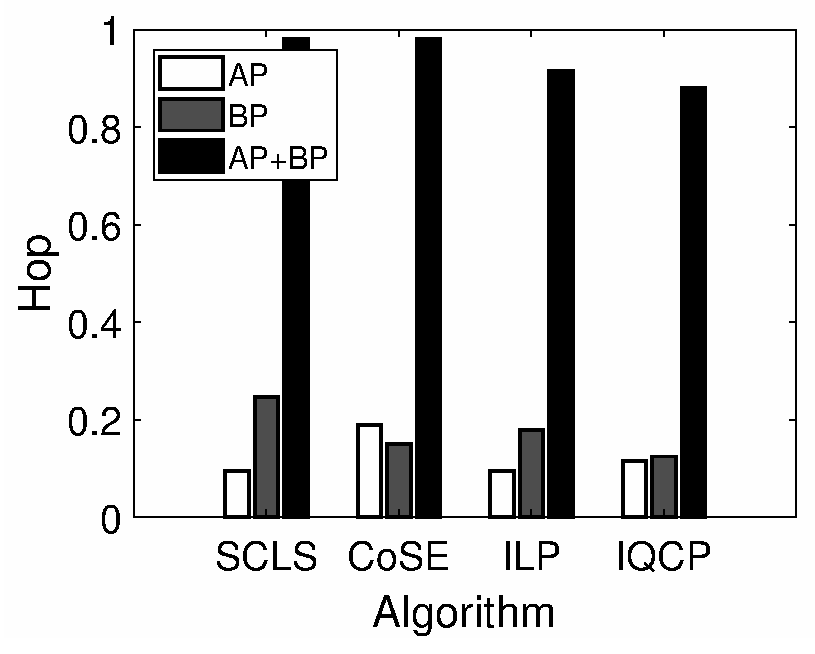
\includegraphics[width=2.25in]{figures/hop}
\caption{路径跳数}
\label{fig:normalization hop}
\end{minipage}
\end{figure}

\end{frame}





\begin{frame}
\begin{figure}[htbp]
\centering
\begin{minipage}[t]{0.3\linewidth}
\centering
\includegraphics[width=1.7in]{figures/runtime}
\caption{运行时间}
\label{fig:normalization runtime}
\end{minipage}
\hfill
\begin{minipage}[t]{0.3\linewidth}
\centering
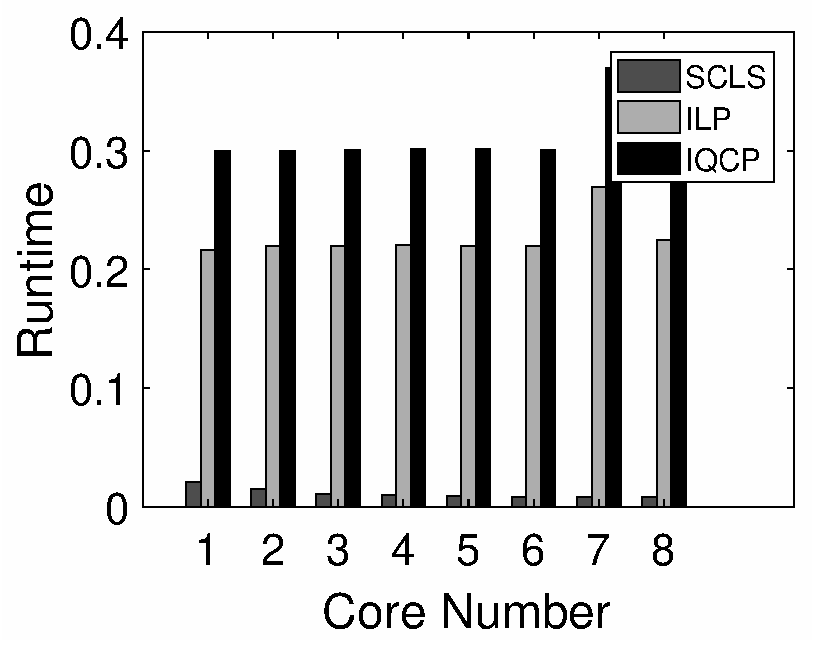
\includegraphics[width=1.7in]{figures/Runtime_noKSP_noCOSE}\\
  \caption{运行时间(无CoSE)}\label{fig:Runtime_noKSP_noCOSE}
\end{minipage}
\hfill
\begin{minipage}[t]{0.3\linewidth}
\centering
\includegraphics[width=1.7in]{figures/speedup}
\caption{核加速比}
\label{fig:Speedup}
\end{minipage}
\end{figure}
\end{frame}

\begin{frame}
\begin{figure}[htbp]
\centering
\begin{minipage}[t]{0.3\linewidth}
\centering
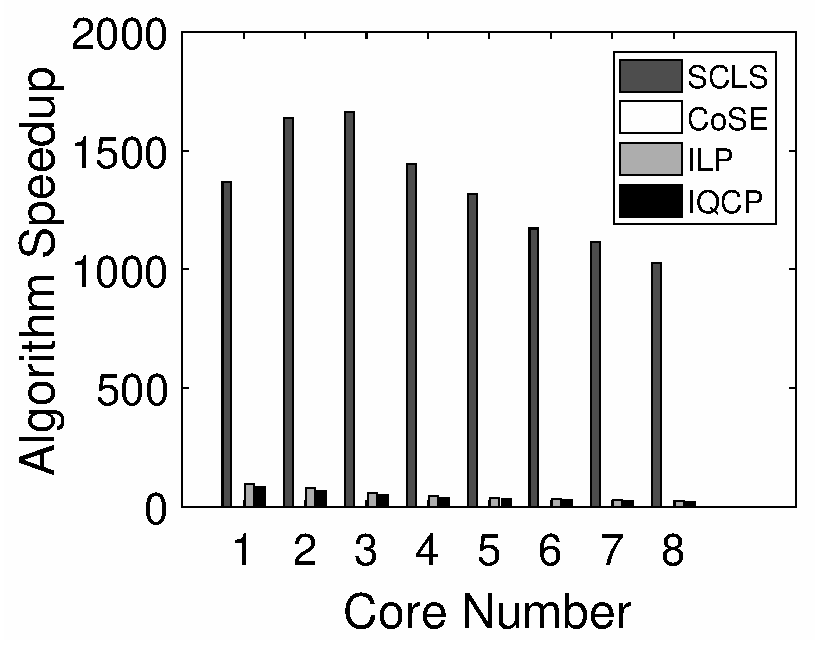
\includegraphics[width=1.7in]{figures/Multiple}
\caption{算法加速比}
\label{fig:Multiple}
\end{minipage}
\hfill
\begin{minipage}[t]{0.3\linewidth}
\centering
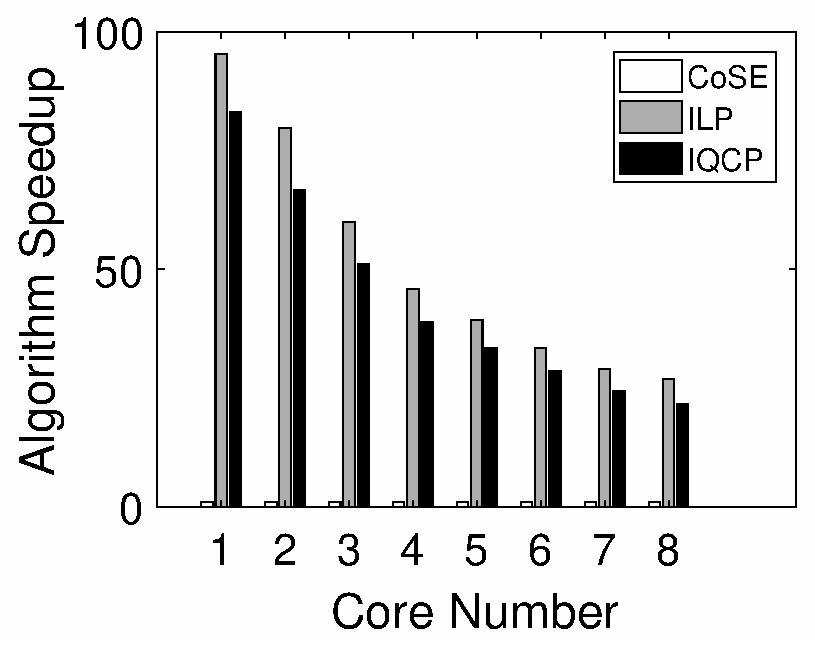
\includegraphics[width=1.7in]{figures/MultipleNoSCLS}
\caption{算法加速比(无SCLS)}
\label{fig:MultipleNoSCLS}
\end{minipage}
\hfill
\begin{minipage}[t]{0.3\linewidth}
\centering
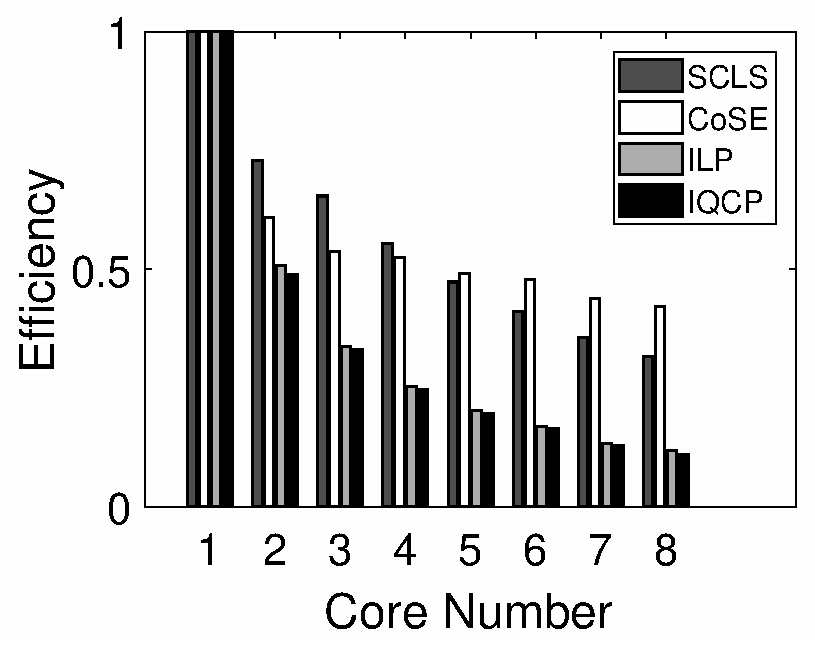
\includegraphics[width=1.7in]{figures/Efficiency}
 \caption{效率}
 \label{fig:Efficiency}
\end{minipage}
\end{figure}
\end{frame}

\section{物理节点单故障可生存性虚拟网络嵌入问题}
\subsection{问题描述}

\begin{frame}{目录}
    \setbeamertemplate{section in toc}[sections numbered]
    \tableofcontents[currentsection,hideothersubsections]
\end{frame}
\addtocounter{framenumber}{-1}  %目录页不计算页码

\begin{frame}
\frametitle{虚拟网络请求}
\textbf{虚拟网络}VN表示为无向图$G (V,E)$,其中$V$ 和$E$ 分别是虚拟节点和虚拟链路的集合。每个虚拟链路$e_{ij}$具有带宽需求$d_{ij}$。 每个虚拟节点$v_i$ 具有计算容量需求$d_i$。 对于虚拟节点$v_i$,需要在虚拟节点上执行的虚拟功能表示为$f(i)$。
\begin{figure}[htbp]
\centering
% Requires \usepackage{graphicx}
\includegraphics[width=1.9in]{figures/VirtualNetworkRequest}\\
\caption{虚拟网络请求$G(V,E)$
}\label{fig:VirtualNetworkRequest}
\end{figure}
\end{frame}

\begin{frame}
\frametitle{底层物理网络}
\textbf{物理网络}建模为一个无向图$G (S,L)$,其中$S$ 和$L$ 分别是物理节点和物理链路的集合。对于物理节点$s_i$,我们使用$F(i)$ 和$c_i$分别表示可以在该节点上执行的一组可行的虚拟功能和可用的计算能力。每个物理链路$l_{ij}$ 都有可用带宽$b_{ij}$。
\begin{figure}[htbp]
\centering
% Requires \usepackage{graphicx}
\includegraphics[width=3.0in]{figures/PhysicalNetwork}\\
\caption{底层物理网络$G(S,L)$}\label{fig:PhysicalNetwork}
\end{figure}
\end{frame}


\begin{frame}
\frametitle{虚拟网络嵌入}
给定VN请求$G (V,E)$情况下,虚拟网络嵌入问题的目的是将该请求映射到物理网络$G (S,L)$ 上,同时提供所需的足够资源。可行的嵌入应该满足节点容量约束、链路带宽约束和功能类型约束这三个约束条件。
\begin{figure}[htbp]
\centering
% Requires \usepackage{graphicx}
\includegraphics[width=2in]{figures/VirtualNetworkEmbedding}\\
\caption{虚拟网络嵌入}\label{fig:VirtualNetworkEmbedding}
\end{figure}
\end{frame}

%\begin{frame}
%  对于VN请求$G (V,E)$和物理网络$G (S,L)$,给出了其占用物理网络的可行映射,在任何一个物理节点发生故障时,增加最小备份物理资源以提供可生存性的网络服务。
%
%  NP-hard?? ILP很难解
%\end{frame}

\subsection{原有算法}
\begin{frame}
\frametitle{原有算法}
\begin{enumerate}
  \item $\SecondAlgorithmMethodAbrreviation$ :算法将备份节点与关键节点之间、备份节点与备份节点之间的连接起来,而不连接关键节点与关键节点之间,关键节点表示嵌入物理节点中的虚拟节点,备份节点表示增广节点。
  \item $\FouthAlgorithmMethodAbrreviation$:1+1-保护机制,当与虚拟节点映射的底层物理上的每个节点失效时,一种简单的方法是增加一个新的物理节点,用于迁移失败的虚拟节点,并将新的链路与失败的物理节点连接起来。
\end{enumerate}
\end{frame}
\begin{frame}

\begin{figure}[htbp]
\centering
\includegraphics[width=3.8in]{figures/One2OneProtection}\\
\caption{1+1-保护机制}\label{fig:One2OneProtection}
\end{figure}
\end{frame}

\subsection{星型图分解动态规划节点嵌入算法}
\subsubsection{基于星型图的分解}
\begin{frame}
\frametitle{设计思想}
\begin{itemize}
  \item 保证局部拓扑结构来保证全部拓扑结构,提出分解原图的方法。
  \item 每个局部结构之间需要协调。
  \item 通过动态规划来实现节点的映射问题。
\end{itemize}

\end{frame}

%\begin{frame}
%\frametitle{星型图定义}
%\begin{equation}
%VirtualStar(v_i)=(v_i, \phi(v_i), d_i, f_i, D_i, N_i)
%\label{eq:virtualstar}
%\end{equation}
%\begin{equation}
%PhysicalStar(s_j)=(s_j, \phi^{-1}( s_j), c_j, F(j), \phi(N(\phi^{-1}( s_j))), a)
%\label{eq:physicalstar}
%\end{equation}
%\end{frame}

\subsubsection{构建星型二分图}
\begin{frame}
\frametitle{构建星型二分图}
  \begin{figure}
\centering
% Requires \usepackage{graphicx}
\includegraphics[width=3.0in]{figures/StarRepresentation}\\
  \caption{当物理节点$s_1$ 失效时VirtualStar($v_i$)和PhysicalStar($s_j$)}\label{fig:StarRepresentation}
\end{figure}
\begin{equation}
VirtualStar(v_i)=(v_i, \phi(v_i), d_i, f_i, D_i, N_i)
\label{eq:virtualstar}
\end{equation}
\begin{equation}
PhysicalStar(s_j)=(s_j, \phi^{-1}( s_j), c_j, F(j), \phi(N(\phi^{-1}( s_j))), a)
\label{eq:physicalstar}
\end{equation}
\end{frame}

%\begin{frame}
%\frametitle{二分图权值设置}
%公式\ref{eq:edge weight}所示在两种不同的情况下定义了边权重$w(i,j)$。
%\begin{equation}
%w(i,j) = \left\{ {\begin{array}{*{20}{c}}
%   { \alpha \sum\limits_{\phi ({v_k}) \notin \phi (N({\phi ^{ - 1}}({s_j})))} {{d_{ik}}} } & {{v_i} \in {\phi ^{ - 1}}({s_j}),v_k \in N(i)}  \\
%   {\alpha \sum\limits_{k \in N(i)} {{d_{ik}}}  + \beta {M_m} + \lambda {c_i} + \theta } & {{v_i} \notin {\phi ^{ - 1}}({s_j}),v_k \in N(i)}  \\
%\end{array}} \right.
%\label{eq:edge weight}
%\end{equation}
%在公式.(\ref{eq:edge weight})中,$\theta$ 被定义如下.
%\begin{equation}
%\theta  = \left\{ {\begin{array}{*{20}{c}}
%   {{C_s}} & {a = 0}  \\
%   0 & {a = 1}  \\
%\end{array}} \right.
%\end{equation}
%\end{frame}

\begin{frame}
\frametitle{多背包问题定义}
\begin{equation}
\huge{
\begin{array}{*{20}{c}}
   {\mathop {\min }\limits_{{M_{ij}}} } & {\sum\limits_{i = 1}^n {\sum\limits_{j = 1}^m {{M_{ij}}{w_{ij}}} } }  \\
   {s.t.,} & {\sum\limits_{i = 1}^n {{d_i}{M_{ij}}}  \le {c_j}}  \\
   {} & {\sum\limits_{j = 1}^m {{M_{ij}}}  \le 1}  \\
   {} & {{M_{ij}} = \{ 0,1\} }  \\
\end{array}
}
\label{eq:problem formulation}
\end{equation}
\end{frame}

\subsubsection{动态规划节点嵌入}

%\begin{frame}
%
%在等式\ref{eq:place i to j}中,如果物理节点$x_j$的容量限制大于容量需求$d_i$ 并且在物理节点${f_i} \in {F_j}$能执行虚拟功能$f_i$,则 $\theta (i,j)$ 是已经放置前面i−-1 个最佳虚拟星型图的代价和(即$dp[i-1][{x_1} - {d_i}][{x_2}] \ldots [{x_m}]$) 和将虚拟星型图($v_i$) 映射到物理星型图($s_1$)的成本(即$w_{i1}$)。基于$\theta (i,j)$,$dp[i][{x_1}][{x_2}] \ldots [{x_m}]$可通过以下动态规划函数计算。
%\begin{equation}
%dp[i][{x_1}][{x_2}] \ldots [{x_m}] = min\{\theta (i,1),\theta (i,2),\ldots,\theta (i,j),\ldots,\theta (i,m)\}
%\label{eq:update function}
%\end{equation}
%\end{frame}
%
%\begin{frame}
%第$i$个虚拟节点可以选择放置在任何一个存活的的物理星型图上。设$\theta (i,j)$ 表示已经将原先$i-1$个虚拟节点最佳放置后再将第$i$ 个虚拟节点放置到第j 个物理节点的备份资源成本。$\theta (i,j)$表示如下:
%\begin{equation}
%\theta (i,j) = \left\{ {\begin{array}{*{20}{c}}
%{dp[i - 1][x_1][{x_2}] \ldots [{x_j} - {d_i}] \ldots [{x_m}] + {w_{ij}}}\\
%\infty
%\end{array}} \right.\begin{array}{*{20}{c}}
%{({x_j} \ge {d_i},{f_i} \in {F_j})}\\
%{otherwise}
%\end{array}
%\label{eq:place i to j}
%\end{equation}
%\end{frame}


\begin{frame}
\frametitle{多背包问题动态规划解法}
\begin{figure}[htbp]
\centering
% Requires \usepackage{graphicx}
\includegraphics[width=4.5in]{figures/DPIllustration}\\
  \caption{动态规划方法的演示}\label{fig:DPIllustration}
\end{figure}
\end{frame}

\begin{frame}
\begin{algorithm}[H]
\label{alg:DPAlg}
\caption{基于动态规划方法二分星型图匹配算法}
\tiny{
\begin{algorithmic}[1]
\REQUIRE {$dp[i][{x_1}][{x_2}] \ldots [{x_m}]=0(1\leq i \leq n, 0\leq x_1\leq c_1, 0\leq x_2\leq c_2,\ldots, 0\leq x_m\leq c_m)$ 首先被定义成无穷大$\infty$,$dp[0][{x_1}][{x_2}] \ldots [{x_m}]=0(0\leq x_1\leq c_1, 0\leq x_2\leq c_2,\ldots, 0\leq x_m\leq c_m)$, m:物理节点的数量。 $M[{x_1}][{x_2}] \ldots [{x_m}]=\textbf{0}_{n\times m}$ 每个节点的映射矩阵}
\ENSURE {当节点容量为$c_1,c_2,\ldots,c_m$时最小代价的节点映射}
\FORALL{$i$ such that $1\leq i\leq n$ }
\FORALL{$x_1,x_2,\ldots,x_m$ such that $ c_1\geq x_1\geq d_i$, $c_2\geq x_2\geq d_i$,$c_3\geq x_3\geq d_i$,$c_m\geq x_m\geq d_i$}
\STATE{$dp[i][{x_1}][{x_2}] \ldots [{x_m}] = min\{\theta (i,1),\theta (i,2),\ldots,\theta (i,j),\ldots,\theta (i,m)\}$}
\STATE{$j' = \mathop {\arg \min }\limits_j \{\theta (i,1),\theta (i,2),\ldots,\theta (i,j),\ldots,\theta (i,m)\}$, }.
\STATE{$M[{x_1}][{x_2}] \ldots [{x_m}]=M[{x_1}][{x_2}] \ldots[x_{j'}-d_i]\ldots [{x_m}]$}
\STATE{$M[{x_1}][{x_2}] \ldots [{x_m}]_{ij'}=1$}
\ENDFOR
\ENDFOR
\RETURN{$dp[i][{c_1}][{c_2}] \ldots [{c_m}]$ and $M[{c_1}][{c_2}] \ldots [{c_m}]$}
\end{algorithmic}
}
\end{algorithm}
\end{frame}

\begin{frame}
\frametitle{可生存性虚拟网络嵌入算法}
\begin{algorithm}[H]
\label{alg:SeVNAlg}
\caption{星型图分解动态规划节点嵌入算法}
\tiny{
\begin{algorithmic}[1]
\REQUIRE $G (V,E)$:虚拟网络请求; $G (S,L)$:物理网络。
\ENSURE 生成SeVN并增加资源将SeVN嵌入到底层物理网络中。
\STATE 将虚拟网络$G^V$ 嵌入到底层网络$G^S$中
\STATE 从与此VN嵌入请求对应的SN中提取嵌入的虚拟网络eVN$G\left( {\hat S,\hat L} \right)$
%\STATE AllMinimumCycle($G(V,E)$)
\FORALL{$v_i$ 并且 $v_i\in G\left( {\hat S,\hat L} \right)$}
\STATE  从图 $G\left( {\hat S,\hat L} \right)$中分解 eVN $G\left( {\hat S,\hat L} \right)$ 成两个星型结构集 $VirtualStar(v_i)$ 和 $PhysicalStar(s_j)$
\STATE 构建items根据星型结构集 $VirtualStar(v_i)$.
\STATE 构建knapsacks根据星型结构集$PhysicalStar(s_j)$
\STATE 构建边权值矩阵
\STATE 动态规划方法解决多背包问题
\STATE 添加新节点,连接新的边,重新分配节点计算资源和链路的带宽资源到$G\left( {\hat S,\hat L} \right)$中构建新的$G\left( {\hat S,\hat L} \right)$
\ENDFOR
\STATE 从 $G\left( {\hat S,\hat L} \right)$中嵌入增广资源到物理网络$G(S,L)$
\end{algorithmic}
}
\end{algorithm}
\end{frame}

\subsection{算法性能评估及比较}
%\begin{frame}
%\frametitle{实验仿真}
%%所有仿真都运行在服务器上,服务器配置为Intel(R) Xeon(R) CPU E5-2620 2.00GHz (24 Cores) 和 32.00GB RAM。
%
%%对于任何VN请求,VN节点的数目是由3到10之间的均匀分布随机得到的,每一对虚拟节点都是以概率0.5 随机连接的。VN节点的计算需求从1到5 之间随机分布,并且VN 上的带宽从1到10之间随机分布。
%
%%VN请求的到达服从泊松过程(平均每1时间单位请求15次)。请求的持续时间服从指数分布,平均100个时间单位,高的请求率和较长的租用时间保证了物理基础设施的高利用率。
%
%%根据\cite{yu2010survivable},即$\lambda/\alpha=\RelativeCostbetweenComputingBandwidth$,节点的计算资源与链路的带宽资源的相对成本为3。 使用的SN 拓扑是SNDlib拓扑数据\cite{orlowski2010sndlib}如表\ref{tab:SNDlibTopo}所示。 底层物理节点(链路)的计算(带宽)资源都是整数的。分别分布在10至20(50 至100)之间。为了对设备节点失效场景进行建模,我们选择了底层物理网络中的所有底层物理设备节点逐个失效,并统计了每$\SubStrateFacilityNodeFailDuration$个时间单元的迁移频率。
%\begin{table}[htb]
%\centering
%\small{
%\caption{SNDlib拓扑数据}\label{tab:SNDlibTopo}
%\begin{tabular}{|c|c|c|}
%  \hline
%  % after \\: \hline or \cline{col1-col2} \cline{col3-col4} ...
%  数据集 & 节点 & 链路 \\
%  \hline
%  cost266& 37& 57\\
%  geant& 22& 36\\
%  germany50& 50& 88\\
%  giul39& 39& 172\\
%  janos-us-ca& 39& 122\\
%  janos-us& 26& 84\\
%  nobel-eu& 28& 41\\
%  norway& 27& 51\\
%  pioro40& 40& 89\\
%  ta1& 24& 55\\
%  ta2& 65& 108\\
%  zib54& 54& 81\\
%  \hline
%
%\end{tabular}
%}
%\end{table}
%\end{frame}



\begin{frame}
\frametitle{接受率}
\begin{figure}[htbp]
\centering
\begin{minipage}{0.4\textwidth}
\centering
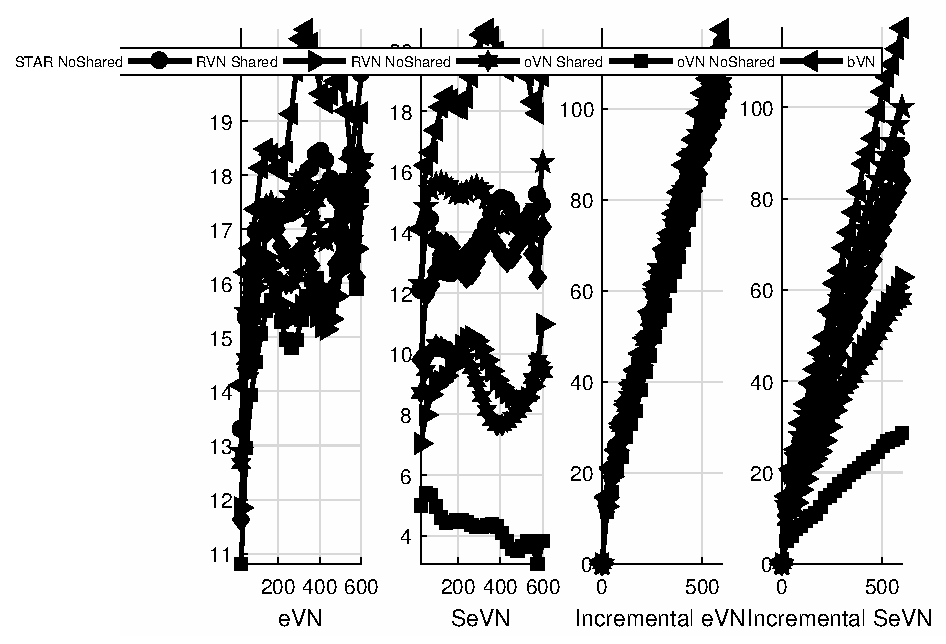
\includegraphics[width=\textwidth]{figures/VirNetReqSurNetReq}
\caption{成功的VNE请求数和成功的SVNE请求数}\label{fig:VirNetReqSurNetReq}
\end{minipage}
\begin{minipage}{0.4\textwidth}
\centering
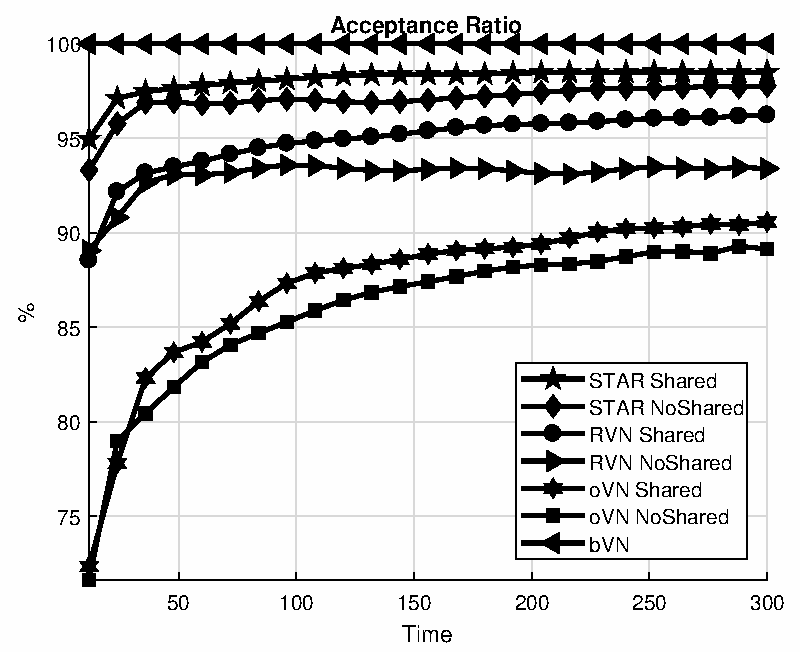
\includegraphics[width=\textwidth]{figures/AcceptionRatio}
\caption{接受率}\label{fig:AcceptionRatio}
\end{minipage}\vspace{\baselineskip}
\end{figure}
\end{frame}


\begin{frame}
\frametitle{活动节点}
\begin{figure}[htbp]
\centering
\begin{minipage}{0.4\textwidth}
\centering
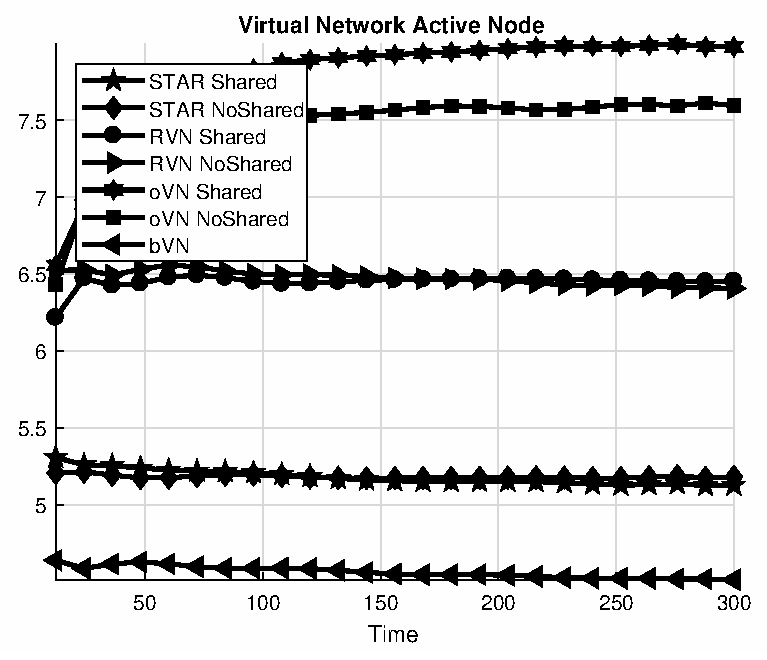
\includegraphics[width=\textwidth]{figures/ActiveNodeAverageVirtualNetwork}
\caption{虚拟网络的平均虚拟节点数}\label{fig:ActiveNodeAverageVirtualNetwork}
\end{minipage}
\begin{minipage}{0.4\textwidth}
\centering
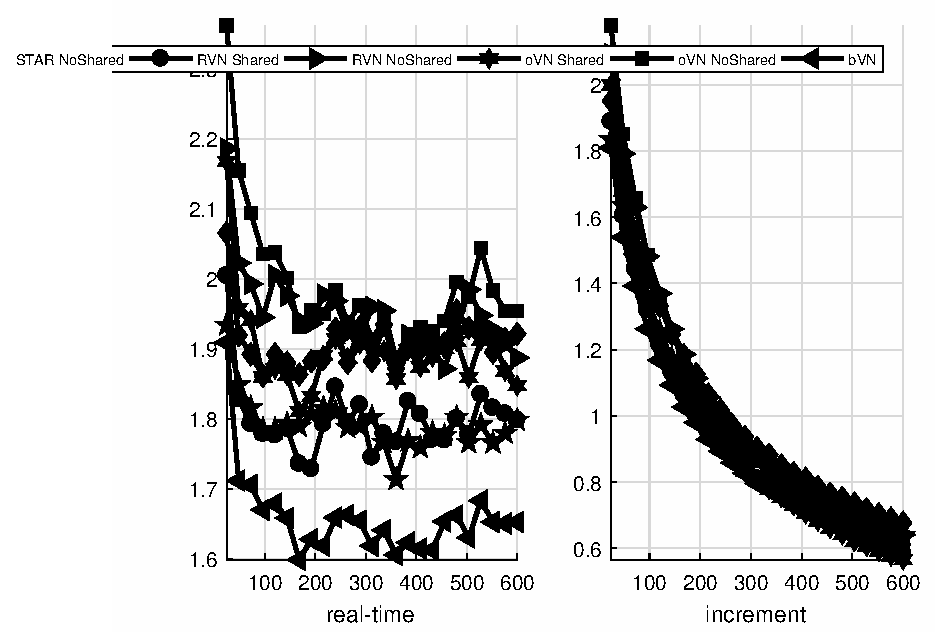
\includegraphics[width=\textwidth]{figures/ActiveNodeAverageSubstrateNetwork}
\caption{底层物理网络平均启动的节点数}\label{fig:ActiveNodeAverageSubstrateNetwork}
\end{minipage}
\begin{minipage}{0.4\textwidth}
\centering
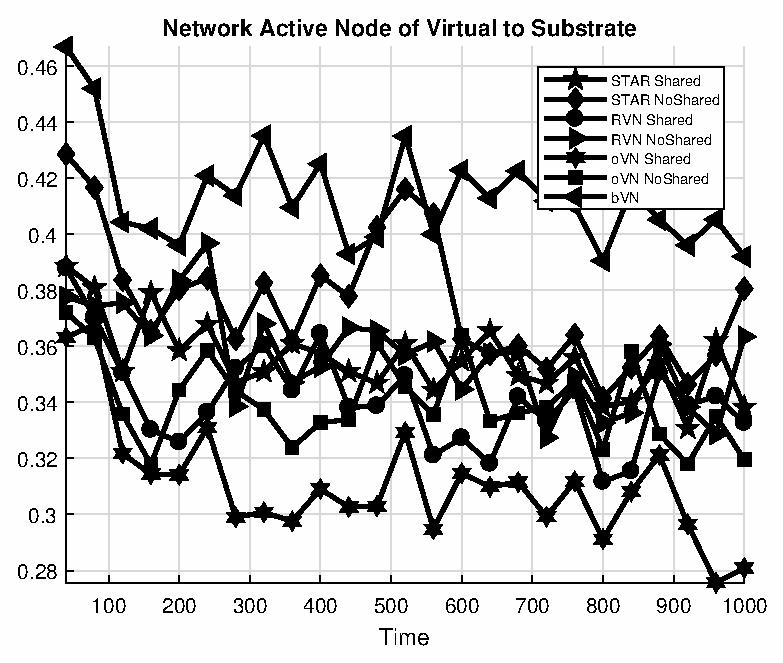
\includegraphics[width=\textwidth]{figures/ActiveNodeSubVir2VirNet}
\caption{底层物理网络启动的节点数与虚拟网络虚拟节点数之比}\label{fig:ActiveNodeSubVir2VirNet}
\end{minipage}\vspace{\baselineskip}
\end{figure}
\end{frame}

\begin{frame}
\frametitle{路径长度}
\begin{figure}[htbp]
\centering
\begin{minipage}{0.4\textwidth}
\centering
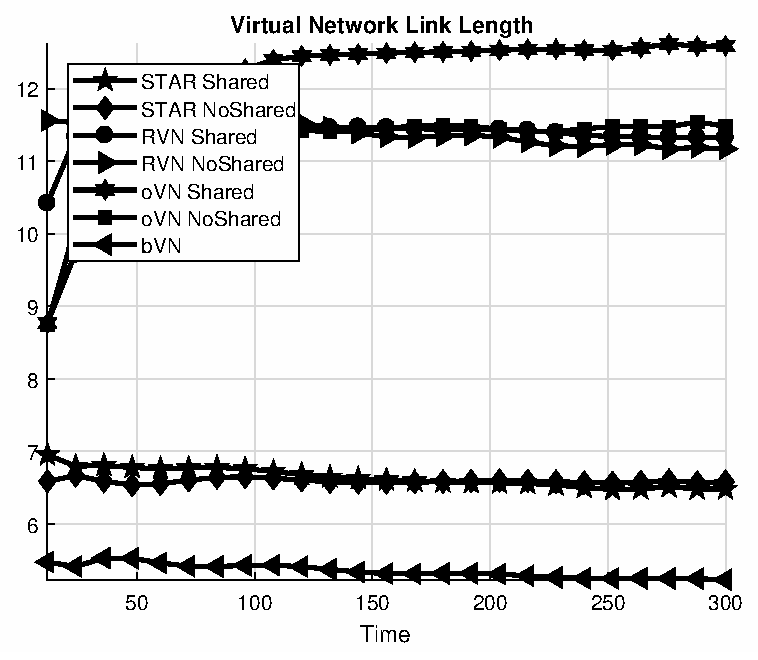
\includegraphics[width=\textwidth]{figures/PathLengthAverageVirtualNetwork}
\caption{虚拟网络链路数}\label{fig:PathLengthAverageVirtualNetwork}
\end{minipage}
\begin{minipage}{0.4\textwidth}
\centering
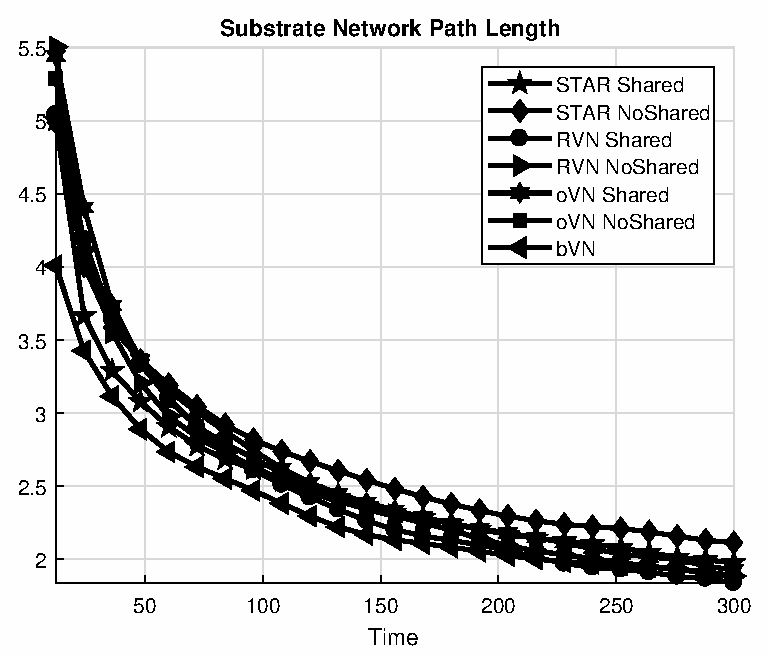
\includegraphics[width=\textwidth]{figures/PathLengthAverageSubstrateNetwork}
\caption{物理网络链路数}\label{fig:PathLengthAverageSubstrateNetwork}
\end{minipage}
\begin{minipage}{0.4\textwidth}
\centering
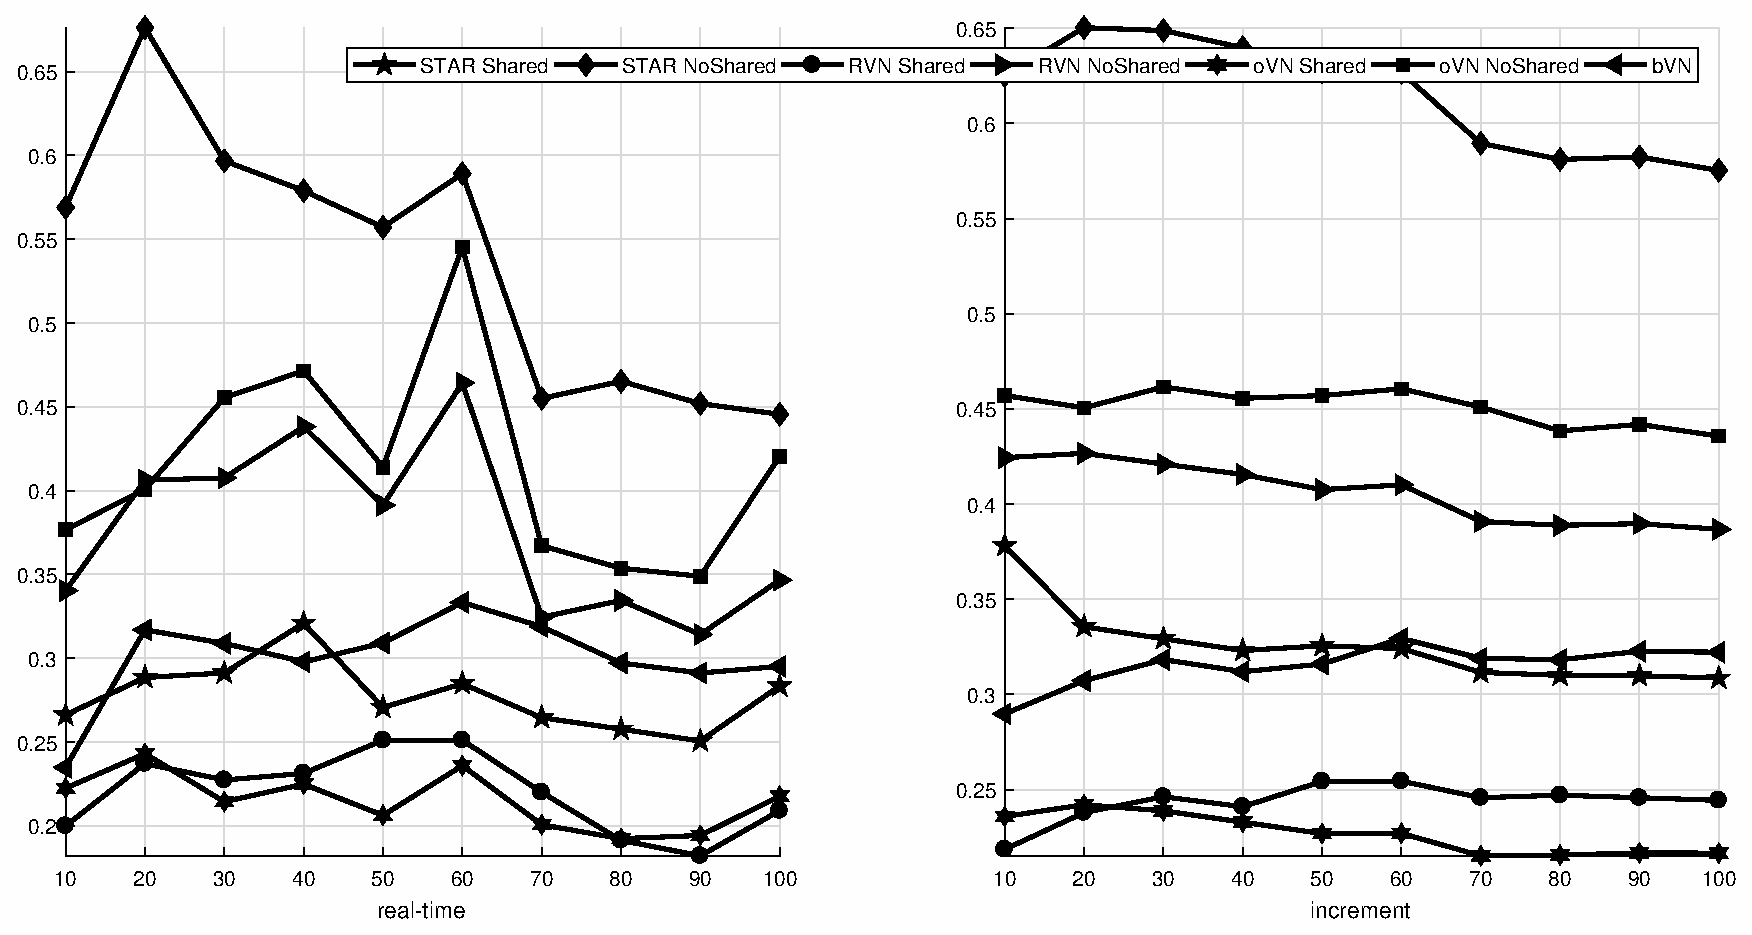
\includegraphics[width=\textwidth]{figures/PathLengthSubVir2VirNet}
\caption{物理网络链路数与虚拟网络链路数之比}\label{fig:PathLengthSubVir2VirNet}
\end{minipage}\vspace{\baselineskip}
\end{figure}
\end{frame}

\begin{frame}
\frametitle{成本与收益}
\begin{figure}[htbp]
\centering
\begin{minipage}{0.4\textwidth}
\centering
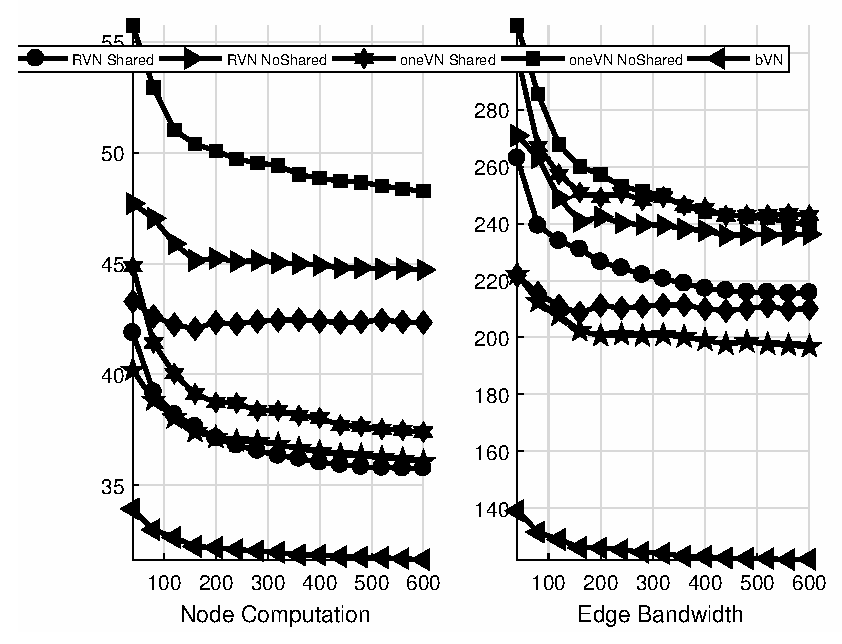
\includegraphics[width=\textwidth]{figures/CostAccumulateAverageSubstrateNetwork}
\caption{底层物理网络消耗资源的平均成本}\label{fig:CostAccumulateAverageSubstrateNetwork}
\end{minipage}
\begin{minipage}{0.4\textwidth}
\centering
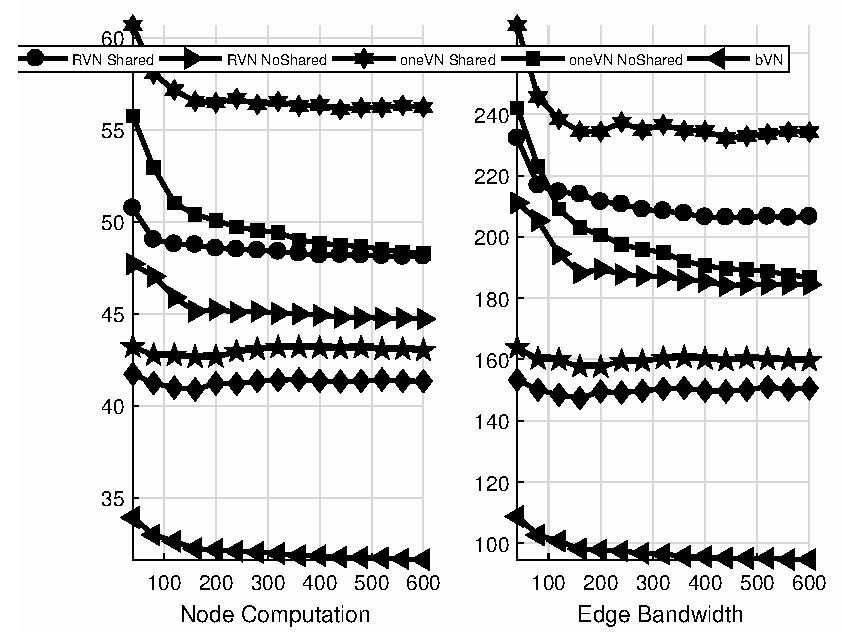
\includegraphics[width=\textwidth]{figures/RevenueAccumulateAverageVirtualNetwork}
\caption{虚拟网络获得需求的平均收益}\label{fig:RevenueAccumulateAverageVirtualNetwork}
\end{minipage}\vspace{\baselineskip}
\end{figure}
\end{frame}

\section{总结}
%\subsection{本文工作总结}
\begin{frame}{目录}
    \setbeamertemplate{section in toc}[sections numbered]
    \tableofcontents[currentsection,hideothersubsections]
\end{frame}
\addtocounter{framenumber}{-1}  %目录页不计算页码
  
\begin{frame}
\frametitle{总结}
\begin{enumerate}
  \item 首先,为了提高主路径传输的可生存性,全面研究了现在网络故障存在的各种故障类型的特点,包括主动式和被动式。针对这些故障恢复机制方式,设计了快速的分而治之的快速SRLG不相交路径对算法。
  \item 本文提出了一种拓扑图在存在陷阱问题情况下求解Min-Min SRLG不相交路由问题的高效算法,为了降低搜索的复杂性,我们创新性提出了一种分而治之的解决方案,将原Min-Min SRLG 不相交路由问题划分为多个子问题,该子问题基于从AP路径上遇到陷阱问题时导出的SRLG冲突链路集。我提出的算法利用现有的AP搜索结果SRLG冲突链路集,来并行执行实现更快的路径查找。
  \item 并且本文在一个多核CPU平台上使用合成的拓扑进行了真实的仿真模拟。仿真结果表明,在搜索速度比较下,该算法的查找性能优于其它现有算法。
  \item 其次,我们分析虚拟网络嵌入问题的本质特征,从而提出适合星型分解动态规划节点嵌入的可生存性虚拟网络嵌入算法,以解决原先可生存性虚拟网络嵌入算法无法解决的时间复杂性和低资源利用率等问题。
  \item 本文在可生存性虚拟网络嵌入问题中,引入网络节点带有特定功能类型的限制条件,创新性提出一种星型分解动态规划节点嵌入的启发式算法,在虚拟和物理星型图之间的权重设置上,考虑网络资源的利用率和网络节点开启代价。
  \item   提出的算法能快速的实现虚拟网络嵌入的可生存性需求,仿真结果表明,我提出的算法与其他现有算法效果比,虚拟嵌入可生存性请求的成功率更高,嵌入的物理资源消耗更低,物理资源的利用率更高。
\end{enumerate}
\end{frame}

%\include{body/chap2}
%\include{body/chap3}
%\include{body/chap4}
%\include{body/chap5}
%\include{body/chap6}
\begin{frame}
\textbf{攻读学位期间所发表的学术论文和专利}
\begin{itemize}
  \item Kun Xie, Heng Tao, Xin Wang, Gaogang Xie, Jigang Wen, Jiannong Cao, Zheng Qin. Divide And Conquer For Fast SRLG Disjoint Routing[C]. DSN 2018: International Conference on Dependable Systems and Networks, Luxerbourg(CCF B)已发表。
  \item 陶恒,谢鲲. 一种求完全风险共享链路组分离路径对的方法及系统:中国。已具有国家知识产权局公开号,并已进入实审阶段。
\end{itemize}
\end{frame}


\begin{frame}[standout]
\begin{center}
\huge{谢谢观看}
\end{center}
\begin{center}
研究生生活即将结束,在此,我要感谢所有教导我的老师和一齐成长的同学,他们在我的研究生学生涯给予了很大的帮助。本论文能够顺利完成,要特别感谢我的导师谢鲲老师,感谢各位老师的关心和帮助!
\end{center}
\begin{center}
  恳请各位老师提出宝贵意见!
\end{center}
\end{frame}

% If there are too many of them to fit on the frame,
% you must manually split them among additional frames or use the allowframebreaks option.
\begin{frame}[allowframebreaks]{References}
  \scriptsize
  \bibliographystyle{plain}
  \bibliography{reference}
\end{frame}

\end{document}
